\documentclass[main.tex]{subfiles}

\pagestyle{fancy}
\fancyhf{}
\fancyhead[LE]{\makebox[\pageoffset][l]{\bfseries\thepage}\bfseries\leftmark}
\fancyhead[RO]{\bfseries\rightmark\makebox[\pageoffset][r]{\bfseries\thepage}}

\begin{document}

\section*{Goal}
These experiments will explore the concepts of displacement and velocity by examining position vs. time and displacement vs. time plots. We will use a motion sensor to detect the motion of objects moving towards and away from the sensor. Also, we will look at the difference between average and instantaneous velocity.

\section*{Equipment}
\begin{itemize}
\item
850 Universal Interface
\item
PASCO Capstone Software
\item
Motion Sensor
\item
Two Photogates
\item
Low-friction dynamics track and cart
\item
Cart-mountable picket fence
\item
Masonite targets
\end{itemize}•

\section*{Theory}
\emph{Displacement} describes the motion of an object from one location in space to another. We can represent this mathematically by,
\[
\Delta x = x-x_0,
\]
where $x$ describes our current position, $x_0$ describes our previous position, and $\Delta x$ represents the change in $x.$ If we were to look at how our displacement changes over a certain time interval, we would know another piece of information about our object called \emph{velocity.} We can define an \emph{average} velocity as,
\[
v_{ave} = \frac{x-x_0}{t-t_0}=\frac{\Delta x}{\Delta t},
\]
where $t$ is the time when the object is at position $x$ and $t_0$ is the time at position $x_0.$ While an average velocity works very well when the velocity is constant, if our object's velocity is changing we could be missing out on information by averaging over a large time span.  To compensate for this, we can shorten our time interval to make our average more accurately describe our velocity at a single instant in time. If we keep shortening our time interval until our starting and ending time are infinitesimally close we can get what is called an \emph{instantaneous} velocity. Those with some calculus background will recognize this as a limiting process. Thus, we can write our instantaneous velocity as,
\[
v=\lim_{t\rightarrow t_0}\frac{x(t)-x(t_0)}{t-t_0}=\frac{dx}{dt}.
\]
\section{Setup I: Motion Graph Matching}
\begin{enumerate}
\item
Turn the 850 Universal Interface (850UI) on.
\item
Attach the Motion Sensor into digital inputs 1 and 2. Use channel 1 for the yellow plug and channel 2 for the black one. (Any two adjacent channels can be used but the yellow plug must always be in the one on the right.) Set the Motion Sensor to the ``people" (wide angle) setting.
\item
Open Capstone from the desktop. In the upper left-hand side click on the button labeled ``Hardware Setup."  There should be a picture of the 850UI shown. If not, ask the instructor for help.
\item
For this experiment we want to load a saved workbook from the computer. Open the file titled ``Motion Graph Matching" by clicking 
\includegraphics{Open_Experiment}. The file should be located in ..\textbackslash Documents\textbackslash Phys Lab Files\textbackslash Phys1154.
\item
Place the Motion Sensor on the edge of a table at a place where there is at least 2.5 m of empty room in front of the sensor.
\item
Aim the Motion Sensor at the Masonite board while standing in front of the sensor.
\item
Position the computer monitor so you can see the screen while you move away from the Motion Sensor.  The Motion Sensor puts out 10 pulses each second for 10 seconds.  The Index on the horizontal axis is the number of pulses, so an Index of 10 corresponds to 1 second.
\end{enumerate}

\subsection*{Procedure}
\begin{enumerate}
\item
Each group member should do the following for one Position graph and one Velocity graph.
\item
Stand an appropriate distance (see start position on Position 1--3)(50 cm for Velocity plots)  in front of the Motion Sensor. 
\item
After you click RECORD, there is a three-second countdown before data recording begins. Watch the Ready clock on the bottom of the screen and be ready to move when it reaches zero.  
\begin{center}

\includegraphics[width=0.33\textwidth]{Motion_Sensor}
\end{center}
\item
The Score display will show how closely you match the graph. The closer to 100, the better.
\item
Click RECORD. The Motion Sensor will make a faint clicking noise to tell you it is on and the green LED will flash.
\item
Try to match the graph by moving forward or backward.  The recording will stop automatically after 10 sec.
\item
Repeat the data recording process as many times as you need (time permitting) to get your best match.  Use the white triangle by the Delete Last Run icon at the bottom of the page to delete unwanted runs (too many recorded runs can cause problems with the program).  If you want to examine a previous run, use the black triangle by the Run Select icon in the graph toolbar above the graph.  It is fairly easy to get a score above 95 on the position plots.  The velocity plots are harder and scores above 80 are good.
\item
Repeat the process for Velocity 1--4.
\end{enumerate}•

\subsubsection*{Position plots}
\begin{question}
What does a horizontal line on a position graph mean?
\end{question}
\begin{question}
What is the difference between the parts of the plot with positive slope and the parts with negative slope?
\end{question}
\begin{question}
On the Position 3 plot, what is happening between 5 and 10 seconds (50 to 100 index)?
\end{question}
\subsubsection*{Velocity plots}
\begin{question}
What does a horizontal line on a velocity graph mean?
\end{question}
\begin{question}
What is the difference between the parts of the plot with positive slope and the parts with negative slope?
\end{question}
\begin{question}
Consider the Velocity 2 plot. What is the difference between places where the slope is large and places where the slope is near zero?
\end{question}

\section{Setup II: Looking at Position \& Velocity graphs together}
\begin{enumerate}
\item
We now want to clear all our data and start a new experiment. We can do this by clicking on the ``New Experiment" button 
\includegraphics{New_Experiment} or going to ``File" \textgreater ``New Experiment."
\item
Before we move on we need to tell Capstone that we are using a Motion Sensor again. To do this click on the ``Hardware Setup" button and on the picture of the 850UI click the port that the Motion Sensor is plugged into. (For sensors like the Motion Sensor, always click on the port that the yellow plug is in.) Simply type in ``Motion Sensor" and click on ``Motion Sensor II." If we have done this correctly, there should be a small icon of the Motion Sensor in the picture with two green lines indicating which ports the sensor is plugged into. Click the ``Hardware Setup" again to hide the window.
\item
We want to create a graph for our experiment. To do this, double-click on the button labeled ``Graph" in the toolbar on the right.
\item\label{step:vel_add_position}
To tell Capstone what data to plot, click on the ``\textless Select Measurement\textgreater" button on the vertical axis and select ``Position."
\item
Now we want to also show a velocity plot on the same graph. To do this in the toolbar above the graph, click on this button 
\includegraphics{Add_New_Plot}
 This will add a second graph below our current one.
\item
Repeat the process from step~\ref{step:vel_add_position}, but this time select ``Velocity."
\end{enumerate}•

\subsection*{Procedure}
\begin{enumerate}
\item\label{step:Plotting}
One member of the group should be the target and do the following: Collect data as the target walks away from the motion detector at a constant speed, pauses for a second, and then walks toward the motion detector at a constant speed. This may take several tries. Pick the best attempt and hide the rest. Rescale the data with this button 
\includegraphics{Rescale} to fit the data.
\item
Notice that both graphs are drawn together. Both should have 3 regions corresponding to the 3 movements in Step \ref{step:Plotting}.
\item\label{step:Delta_Tool_Begin}
While the Position graph is selected, click on the Coordinates/Delta Tool 
\includegraphics{Coordinates_Tool} and drag it to a point in the first region.
\item
To get access to the ``Delta Tool," right-click the Coordinates tool in the graph and select ``Tool Properties." Check ``Show Delta" and change the ``Delta Tool Style" to be ``$\Delta y/\Delta x$ with slope.." Click ``Okay" to close the window.
\item
Drag the new tool to another data point along the straight-line portion of our graph. The graph should show a box with $\Delta x/\Delta t =$ value, where the value is the \emph{slope} of the straight line connecting the two points. This is the \emph{average velocity} of our motion between the two times we have selected. Record the midpoint of the time interval and the slope shown in the Delta Tool in the data table.
\item \label{step:Delta_Tool_End}
Now look at the Velocity versus time graph. In the data table, record the same time as you recorded above and the velocity at this time as given on this graph. (Use the Coordinate Tool to display the point.) 
\item
Repeat Steps~\ref{step:Delta_Tool_Begin}--\ref{step:Delta_Tool_End} above for the other straight regions on your graph. \textbf{Print} out a copy of the graph displaying the data in each region (use multiple Coordinate Tools) for all group members. 
\end{enumerate}•

\begin{question}
Taking the velocity from the velocity-vs.-time graph as the standard, calculate the percent discrepancy with the average value of the velocity from the position-versus-time graph for the three cases. 
\[
\%\text{ discrepancy} = \frac{|\text{experimental}-\text{standard}|}{\text{standard}}\times 100\%
\]
\end{question}
\begin{question}
Why are the two values of the velocity from the two graphs not the same? Or, if they are the same, should they be?
\end{question}
\begin{question}
What can you say about the position-versus-time graph when the velocity is negative as shown on the velocity-versus-time graph?
\end{question}

\section{Setup III: Instantaneous Velocity.}
\begin{enumerate}
\item
Disconnect the (real) motion sensor from 850UI and wrap the cord up. Place it aside; out of the way.
\item
Open the file called ``DispVel3." It should be located in ..\textbackslash Documents\textbackslash Phys Lab Files\textbackslash Phys1154.
\item
Place the Photogate connected to Digital Channel 1 (``Gate 1") at the top end of the track 40 cm away from the $X_1$ point. Place the Photogate connected to Digital Channel 2 (``Gate 2") at the bottom end of the track 40 cm away from the $X_1$ point.

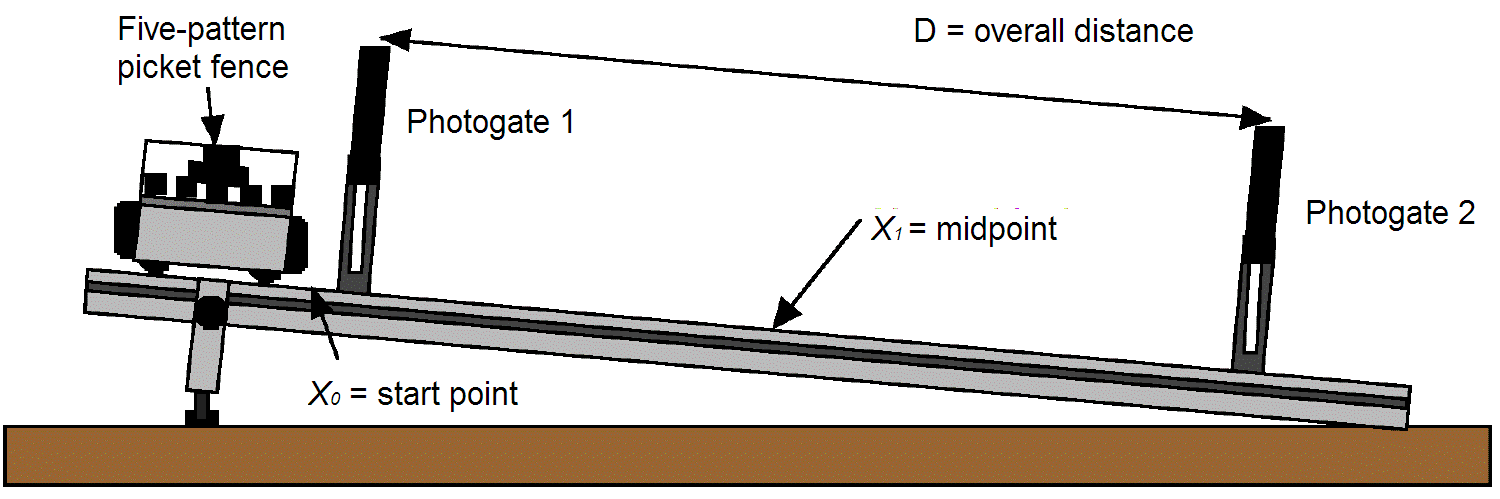
\includegraphics[width=\textwidth]{Disp-Vel_III_Setup}

\item
Place the ``five-pattern picket fence" into the accessory tray on the top of the dynamics cart. Place the picket fence so that \emph{one of the solid bands} will block the Photogate beam as the cart moves down the track. Put the cart on track. Adjust the height of both Photogates so that the Photogate beams are blocked when the cart and picket fence move down the track. Before recording any data for later analysis, you should experiment with the Photogate, cart, and picket fence. Put the cart at the starting point on the track and release it. Do the lights on both Photogates come on? Adjust them as necessary.
\end{enumerate}•

\subsubsection*{Procedure}
\begin{enumerate}
\item
The goal of this section is to determine the instantaneous velocity of the cart at $X_1,$ the midpoint between the two Photogates. You will do this by measuring the \emph{average} velocity of the cart as we progressively reduce the distance between the Photogates.
\item
Record the location of the $X_1$ as indicated by the scale on the track. Check to see that the Photogates are equidistant from this point. Record the initial position of the cart. You will release the cart from this position for every run.
\item
Click on the ``Preview" button to begin the experiment.
\item
Release the cart so it moves down the track. Data recording begins when the Photogate beam is first blocked. If the cart successfully passes through both gates (watch for the lights!), enter the distance between the gates in the table and press the ``Keep Sample" button. Make sure \textbf{not} to click the ``Stop" button as it will stop your current run.
\item \label{step:Vel3_begin}
Move the two Photogates closer to the midpoint X1 by the same amount of distance---say, 5 cm. Adjust the heights of the Photogates above the track so that the cart's picket fence will still block them.
\item \label{step:Vel3_end}
Perform another run at this new position: Release the cart from the same initial position as before. If it passes successfully through both Photogates, enter the new distance in the table and click ``Keep Sample."
\item
Repeat Steps \ref{step:Vel3_begin}--\ref{step:Vel3_end} until the Photogates are as close as possible to $X_1.$
\item
After you have collected the last data, then click on the ``Stop" button. This will end the data run. Make a \emph{Linear} fit~
\includegraphics{Curve_Fit} of the data in the graph. \textbf{Print} out a copy of this graph for each of the group members.
\end{enumerate}

\begin{question}
Which of the average speeds that we measured gives the closest approximation to the instantaneous speed of the cart as it moved through the midpoint $X_1?$ Why?
\end{question}
\begin{question}
What is the relationship between the ``$y$-intercept" on the graph and the instantaneous speed of the cart as it moved through the midpoint $X_1?$
\end{question}
\begin{question}
What factors (accuracy of timing, release of object, accuracy of position measurements, etc.) influence the results? Do errors in these factors produce large changes in your results or small ones? Are the errors random or systematic?
\end{question}
\begin{question}
How does a Photogate work?
\end{question}

\begin{samepage}
\hrulefill\\ \\
\emph{Chapter~\ref{chap:Disp-Vel}:} \textbf{Displacement \& Velocity}
\begin{enumerate}
\item
\textbf{(1)} Title Page --- Title, name, name of lab partners, date of lab.
\item
\textbf{(4)} Purpose --- What was the goal of Displacement \& Velocity III?
\item
\textbf{(10)} Theory --- Discuss what information can be gathered from a position vs. time graph and a velocity vs. time graph. Explain how this information is found. Make sure to include the equations for \emph{both} average and instantaneous velocity.
\item
\textbf{(4)} All graphs.
\item
\textbf{(3)} Data Table.
\item
\textbf{(24)} Answers to all questions.
\item
\textbf{(4)} Conclusion --- What were the findings from Displacement \& Velocity III? How good were they?
\end{enumerate}•
\end{samepage}

\newpage
\begin{doublespace}
\section{Data Table}
\subsection*{Setup II}

\begin{tabular}{|c|c|c|c|c|}
\hline
Region & Midpoint (s) & $v_{ave}$ (m/s) & $v_{inst}$ (m/s) & \% discrepancy\\
\hline
Left &&&&\\
\hline
Center &&&&\\
\hline
Right &&&&\\
\hline
\end{tabular}

\end{doublespace}

\end{document}
